

% This is a simple sample document.  For more complicated documents take a look in the exercise tab. Note that everything that comes after a % symbol is treated as comment and ignored when the code is compiled.

\documentclass{article} % \documentclass{} is the first command in any LaTeX code.  It is used to define what kind of document you are creating such as an article or a book, and begins the document preamble

\usepackage{amsmath} % \usepackage is a command that allows you to add functionality to your LaTeX code
\usepackage{tikz}
\usepackage{enumitem}
\usepackage{varwidth}
\usepackage{tasks}

\usetikzlibrary{automata, positioning}

\title{%
  CW 1.3, Automata. \\
  \large F29LP}
\author{%
Yoav Levi\\
\small H00347035
} % Sets authors name
\date{\today} % Sets date for date compiled

% The preamble ends with the command \begin{document}
\begin{document} % All begin commands must be paired with an end command somewhere
    \maketitle % creates title using information in preamble (title, author, date)
    
    \section{/$(ab)*$/} % creates a section
    \section{/$(b*a)+a+b[ab]*$/}
    \section{NFA}
    \begin{enumerate}
    \item $L=\{w\in \{a,b\}\ast | \text{w contains at most two a's}\}$\\
        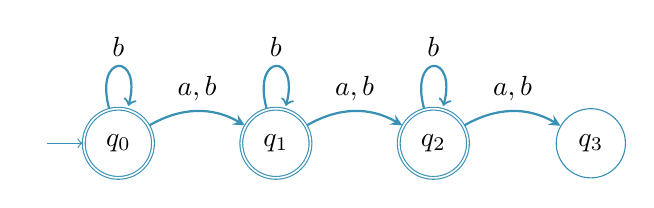
\begin{tikzpicture} [draw=cyan!70!black,
            node distance = 2cm, 
            on grid, 
            auto]
         
            % State q0 
            \node (q0) [state, 
                initial, 
                accepting, 
                initial text = {}] {$q_0$};
            
            % State q1    
            \node (q1) [state,
                accepting, 
                right = of q0] {$q_1$};
            
            % State q2    
            \node (q2) [state,
                accepting,
                right = of q1] {$q_2$};
            
            % State q1    
            \node (q3) [state,
                right = of q2] {$q_3$};
            
            % Arrows
            \path [-stealth, thick]
                (q0) edge[bend left] node {$a,b$}   (q1)
                (q1) edge[bend left] node {$a,b$}   (q2)
                (q2) edge[bend left] node {$a,b$}   (q3)
            
                (q0) edge [loop above]  node {$b$}()
                (q1) edge [loop above]  node {$b$}()
                (q2) edge [loop above]  node {$b$}();
        \end{tikzpicture}
    \item $L=\{w\in \{a,b\}\ast | \text{w contains an even number of occurrences of ab as a subword}\}$\\
        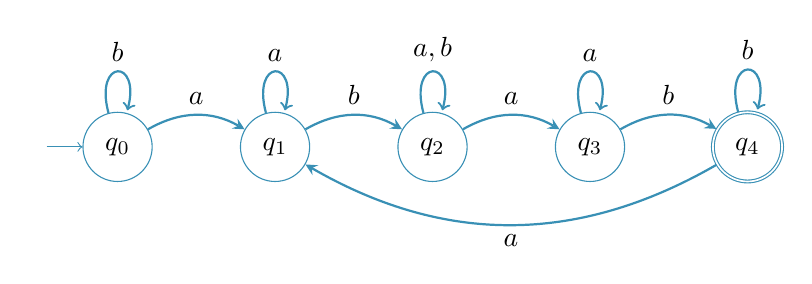
\begin{tikzpicture} [draw=cyan!70!black,
            node distance = 2cm, 
            on grid, 
            auto]
        
        % State q0 
        \node (q0) [state, 
            initial,  
            initial text = {}] {$q_0$};
        
        % State q1    
        \node (q1) [state, 
            right = of q0] {$q_1$};
        
        % State q2    
        \node (q2) [state,
            right = of q1] {$q_2$};
        
        % State q3    
        \node (q3) [state,
            right = of q2] {$q_3$};
        
        % State q4    
        \node (q4) [state,
            accepting,
            right = of q3] {$q_4$};
        
        % Arrows
        \path [-stealth, thick]
            (q0) edge[bend left] node {$a$}   (q1)
            (q1) edge[bend left] node {$b$}   (q2)
            (q2) edge[bend left] node {$a$}   (q3)
            (q3) edge[bend left] node {$b$}   (q4)
            (q4) edge [bend left]  node {$a$} (q1)
        
            (q0) edge [loop above]  node {$b$}()
            (q1) edge [loop above]  node {$a$}()
            (q2) edge [loop above]  node {$a,b$}()
            (q3) edge [loop above]  node {$a$}()
            (q4) edge [loop above]  node {$b$}();
        \end{tikzpicture}
        \newpage
    \item $L=\{w\in \{a,b\}\ast | \text{the first and the last letter of w are identical}\}$\\
        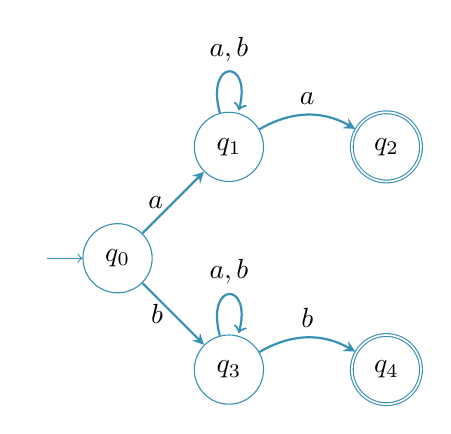
\begin{tikzpicture} [draw=cyan!70!black,
            node distance = 2cm, 
            on grid, 
            auto]
        
        % State q0 
        \node (q0) [state, 
            initial,  
            initial text = {}] {$q_0$};
        
        % State q1    
        \node (q1) [state, 
            above right = of q0] {$q_1$};
        
        % State q2    
        \node (q2) [state,
            accepting,
            right = of q1] {$q_2$};
        
        
        % State q1    
        \node (q3) [state, 
            below right = of q0] {$q_3$};
        
        % State q2    
        \node (q4) [state,
            accepting,
            right = of q3] {$q_4$};
        
        % Arrows
        \path [-stealth, thick]
            (q0) edge [left] node {$a$} (q1)
            (q0) edge [left] node {$b$} (q3)
            (q1) edge [bend left] node {$a$} (q2)
            (q3) edge [bend left] node {$b$} (q4)
        
            (q1) edge [loop above]  node {$a,b$}()
            (q3) edge [loop above]  node {$a,b$}()
            ;
        \end{tikzpicture}
    \end{enumerate}
    \section{/$a*(ba\{2,\})*$/}
    \section{}
            \begin{gather*}
                S \to aA\\
                A \to aB\\
                B \to aS | aC\\
                C \to S | \epsilon
            \end{gather*}
    \section{Unmarked, N/A}
    \section{}
        \begin{enumerate}

            \item
            \begin{gather*}
                S \to aA | bB\\
                A \to aA | bS | aB | \epsilon\\
                B \to aS
            \end{gather*}
            \item Is ambiguous as "aaaa" can be constructed in two ways
            \begin{center}
                \begin{varwidth}{\textwidth}
                \begin{tasks}[label={(\Roman*)},label-width={1cm}](2)
                    \task
                    \begin{tabular}{ c c}
                        Rule & Result\\
                        $S \to aA$ & a\\
                        $A \to aA$ & aa\\
                        $A \to aA$ & aaa\\
                        $A \to aA$ & aaaa\\
                        $A \to \epsilon$ & $\underline{aaaa}$
                    \end{tabular}

                    \task
                    \begin{tabular}{ c c}
                        Rule & Result\\
                        $S \to aA$ & a\\
                        $A \to aB$ & aa\\
                        $B \to aS$ & aaa\\
                        $S \to aA$ & aaaa\\
                        $A \to \epsilon$ & $\underline{aaaa}$
                    \end{tabular}
                \end{tasks}
                \end{varwidth}
            \end{center}
        \end{enumerate}
    \section{ The CFG is used to create a number of a's with an equivalent number of b's, in any order.}

\end{document} % This is the end of the document
